\documentclass[11pt]{article}
\usepackage[margin=1in]{geometry}
\usepackage{booktabs}
\usepackage{graphicx}
\usepackage{amsmath,bm}
\usepackage{caption}

\title{PROM-first master-ANN diagnostic}
\date{}

\begin{document}
\maketitle

\section*{Setup}
This note analyzes the PROM-first version of the master ANN experiment.  The
linear PROM with $n_{\mathrm{tot}}=151$ is used as the coefficient reference.
The case $n=0$ denotes the purely data-driven prediction
$\mathbf q_{\mathrm{tot}}=\mathcal G(\bm\mu,t)$, while intermediate Case~2
runs solve the first $n$ PROM coordinates and inject the remaining
coordinates from the same master ANN:
\[
\widetilde{\mathbf u}
=
\mathbf u_{\mathrm{ref}}
+\mathbf V_{1:n}\mathbf q_{1:n}
+\mathbf V_{n+1:151}\mathcal G_{n+1:151}(\bm\mu,t).
\]
This file is separate from the manuscript and is meant only to inspect the
current PROM-level evidence.

\section*{Case 2 sweep in solved PROM dimension}
The following tables and figures show how the state error and the full
coefficient-trajectory error vary as the number of solved coordinates grows
from the data-driven limit ($n=0$) to the linear PROM reference ($n=151$).

\begin{center}
\small
\begin{tabular}{rccccc}
\toprule
$n$ & $\mu^{(v)}$ & $\mu^{(1)}$ & $\mu^{(2)}$ & $\mu^{(3)}$ & Mean \\
\midrule
0 & 1.036\% & 1.675\% & 1.842\% & 3.214\% & 1.942\% \\
3 & 1.125\% & 1.816\% & 2.168\% & 5.294\% & 2.601\% \\
5 & 1.143\% & 1.697\% & 2.011\% & 5.157\% & 2.502\% \\
10 & 1.013\% & 1.427\% & 1.670\% & 1.898\% & 1.502\% \\
20 & 0.999\% & 1.328\% & 1.505\% & 1.658\% & 1.373\% \\
30 & 0.986\% & 1.283\% & 1.438\% & 1.609\% & 1.329\% \\
50 & 0.966\% & 1.229\% & 1.324\% & 1.556\% & 1.269\% \\
100 & 0.744\% & 0.858\% & 0.833\% & 1.100\% & 0.884\% \\
151 & 0.413\% & 0.460\% & 0.472\% & 0.868\% & 0.553\% \\
\bottomrule
\end{tabular}
\captionof{table}{State relative error against HDM for the Case~2 $n$-sweep.}
\end{center}

\begin{center}
\small
\begin{tabular}{rccccc}
\toprule
$n$ & $\mu^{(v)}$ & $\mu^{(1)}$ & $\mu^{(2)}$ & $\mu^{(3)}$ & Mean \\
\midrule
0 & 2.499\% & 3.924\% & 4.249\% & 7.444\% & 4.529\% \\
3 & 2.684\% & 4.247\% & 4.955\% & 12.331\% & 6.054\% \\
5 & 2.721\% & 3.975\% & 4.614\% & 11.961\% & 5.818\% \\
10 & 2.440\% & 3.361\% & 3.906\% & 4.257\% & 3.491\% \\
20 & 2.401\% & 3.123\% & 3.512\% & 3.662\% & 3.175\% \\
30 & 2.372\% & 3.020\% & 3.367\% & 3.501\% & 3.065\% \\
50 & 2.319\% & 2.847\% & 3.113\% & 3.256\% & 2.884\% \\
100 & 1.707\% & 1.897\% & 1.859\% & 1.806\% & 1.817\% \\
151 & 0.000\% & 0.000\% & 0.000\% & 0.000\% & 0.000\% \\
\bottomrule
\end{tabular}
\captionof{table}{Full coefficient-trajectory error against the linear PROM reference for the same $n$-sweep.}
\end{center}

\begin{figure}[h!]
\centering
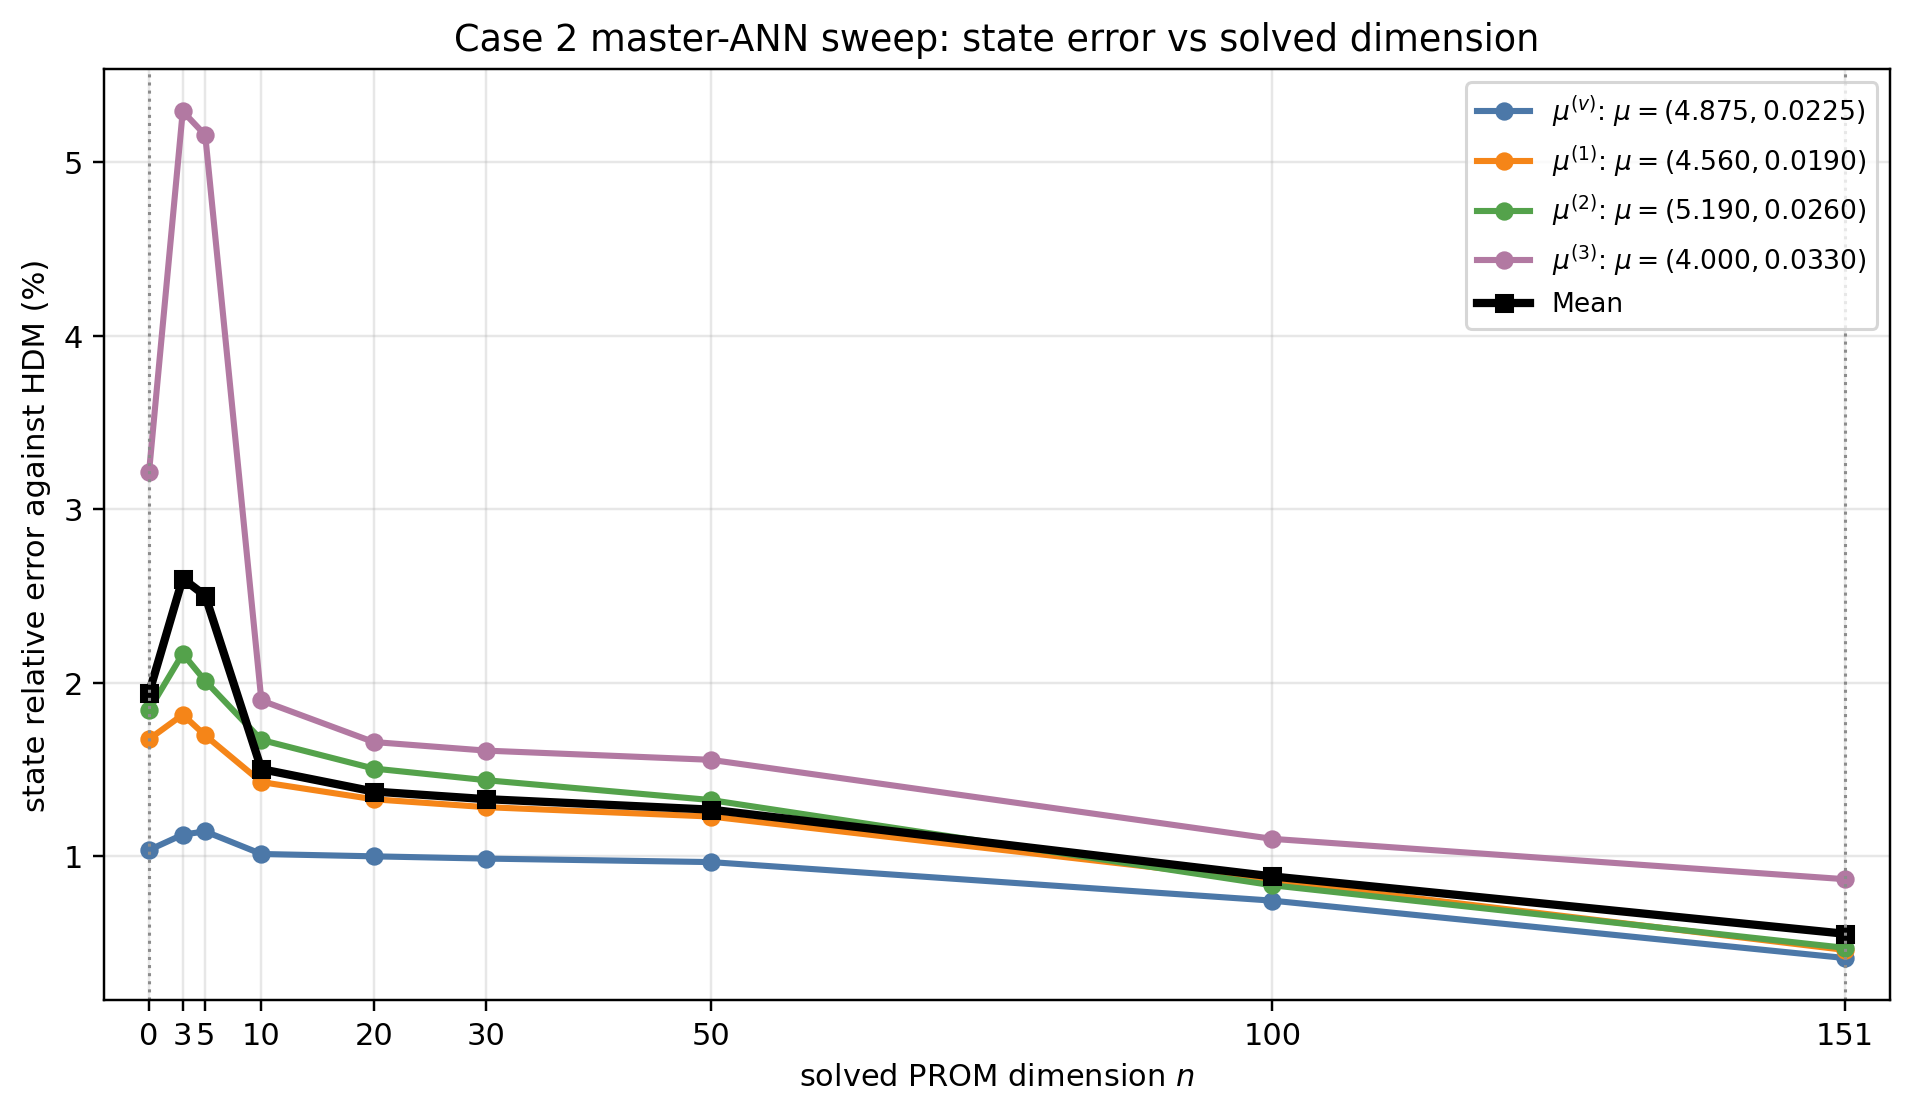
\includegraphics[width=0.88\textwidth]{figures/prom_case2_n_sweep_state_errors.png}
\caption{State relative error against HDM as a function of the number of PROM coordinates solved online.}
\end{figure}

\begin{figure}[h!]
\centering
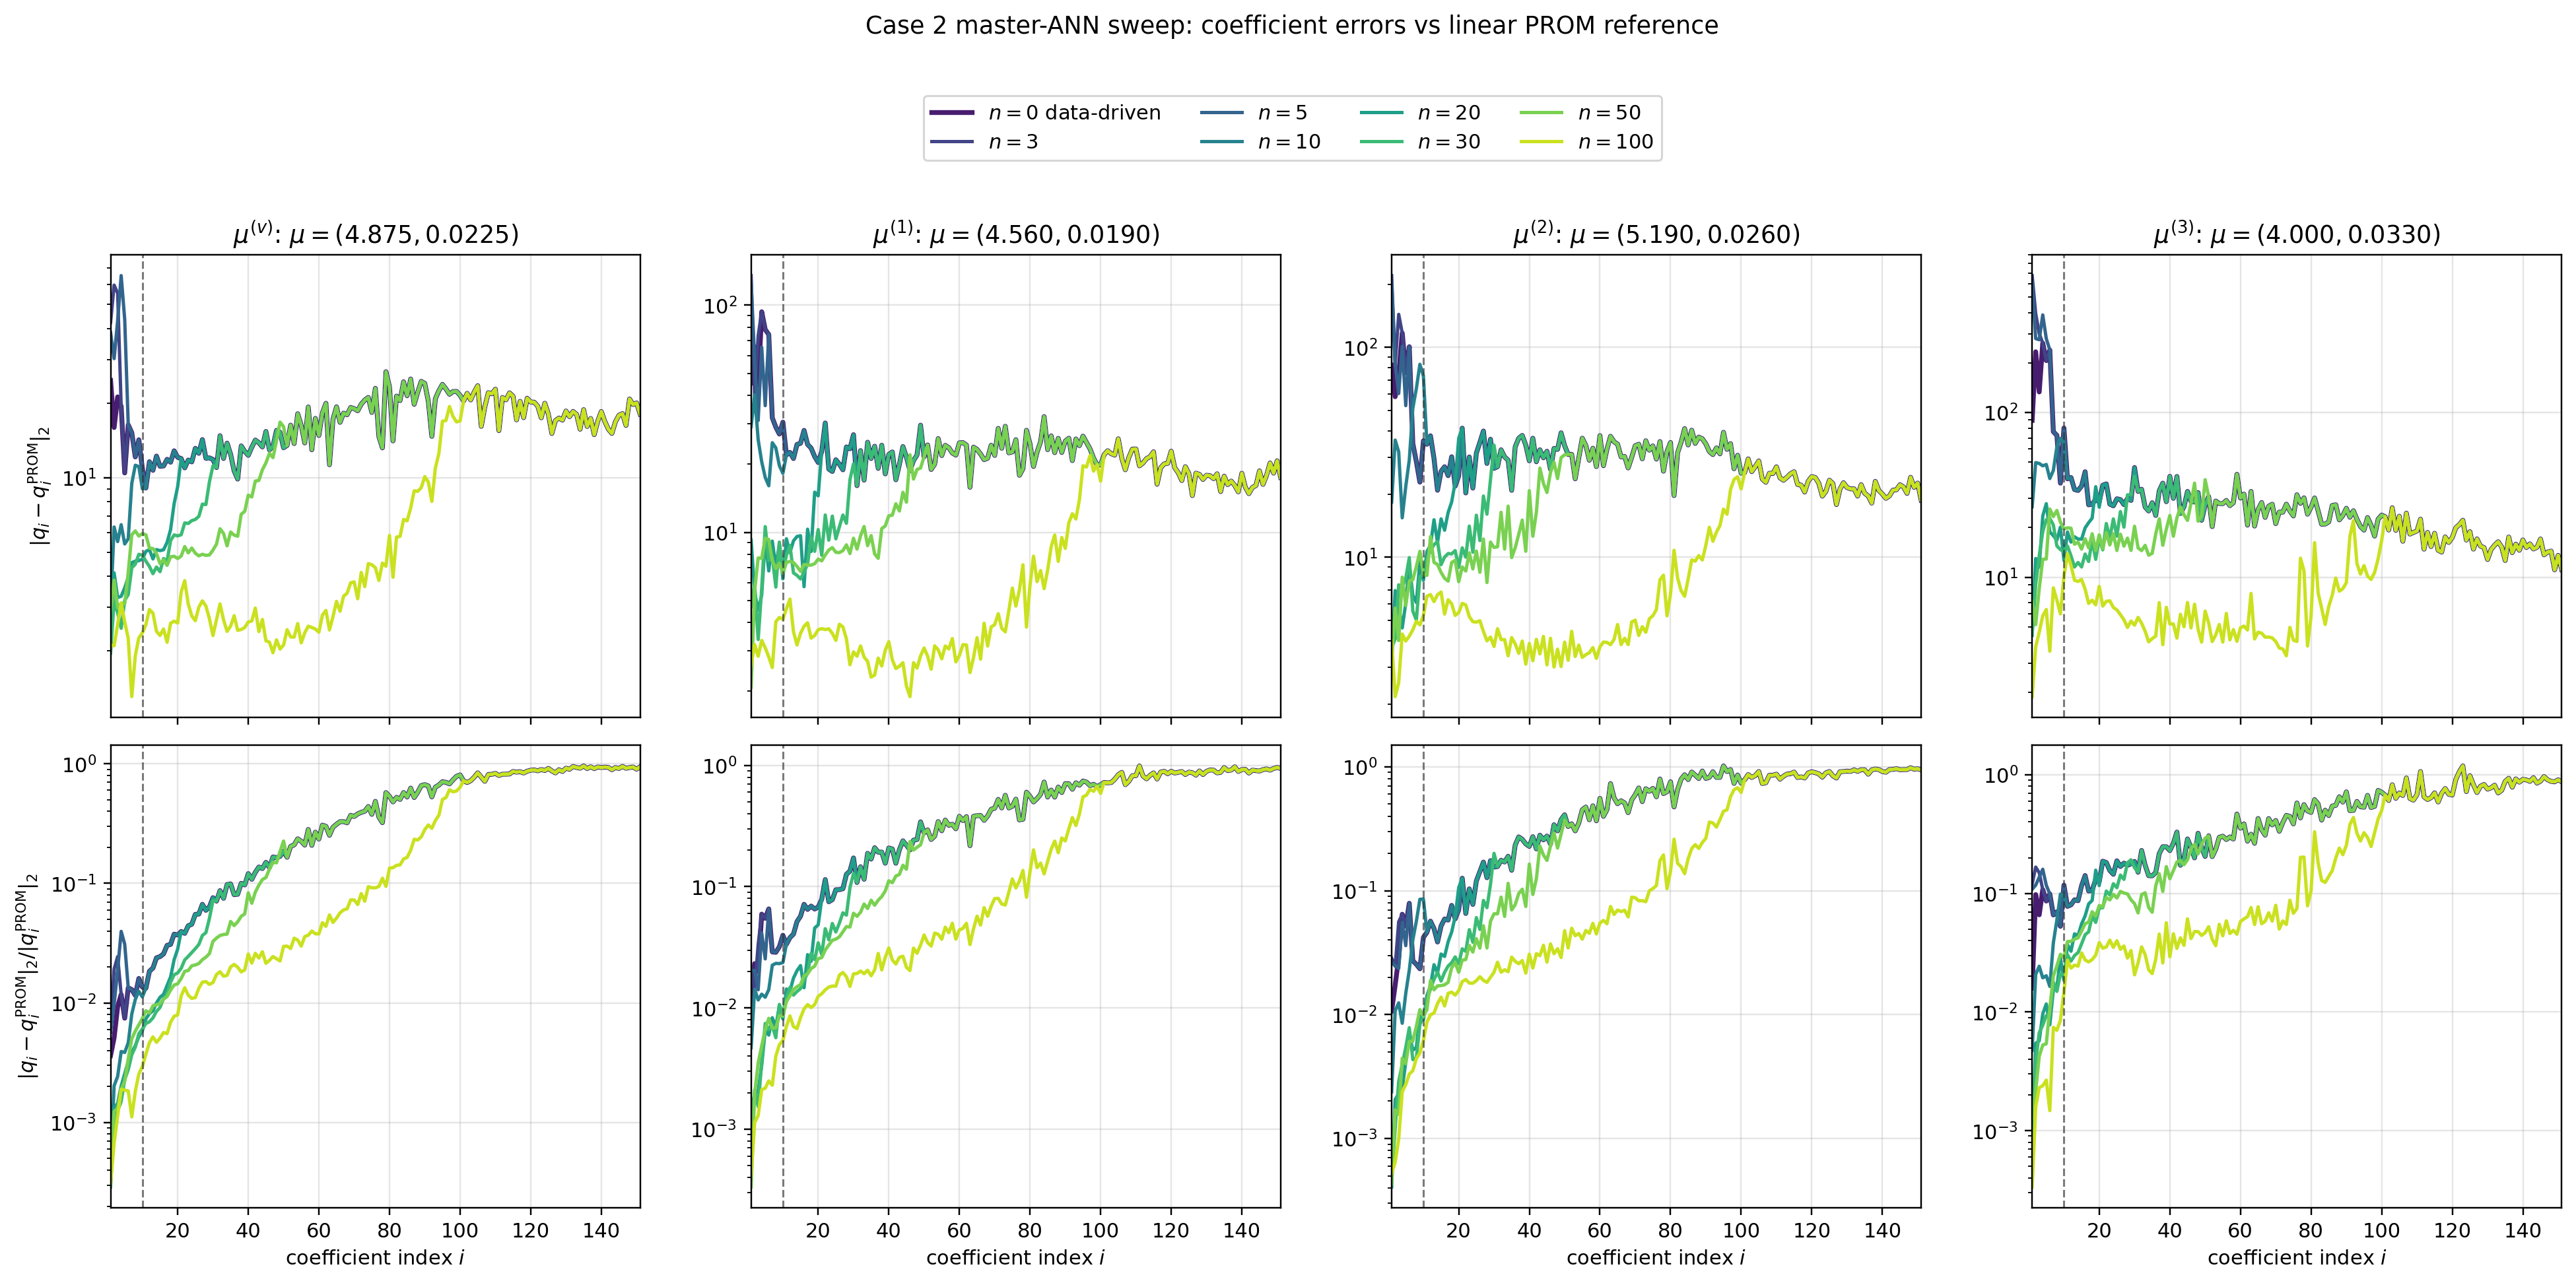
\includegraphics[width=0.98\textwidth]{figures/prom_case2_n_sweep_coeff_abs_rel_all_points.png}
\caption{Per-coefficient absolute and relative errors for the same $n$-sweep.  The linear PROM case $n=151$ is not plotted because it is the zero-error coefficient reference.}
\end{figure}

\clearpage
\section*{Case 2 $n=10$: sensitivity to secondary-coordinate error}
This diagnostic isolates one mechanism in Case~2.  The secondary coordinates
$q_{11},\ldots,q_{151}$ are prescribed from the linear PROM and then perturbed
in the direction of the actual master-ANN error.  The horizontal axis is the
imposed relative error in those prescribed secondary coordinates.  The star on
each curve marks the actual ANN secondary error for that test point.
This is not the global validation error of the ANN.  The trained master ANN has
a full-trajectory validation error of about $4.39\%$ on
$\mathbf q_{\mathrm{tot}}$, whereas the horizontal-axis values here measure
only
\[
\frac{\|q_{11:151}^{ANN}-q_{11:151}^{PROM}\|_F}
{\|q_{11:151}^{PROM}\|_F}
\]
on the four test points.  Since the secondary block carries only about
$20\%$ of the full coefficient norm, this secondary-only relative error can be
much larger than the full $\mathbf q_{\mathrm{tot}}$ error.

\begin{figure}[h!]
\centering
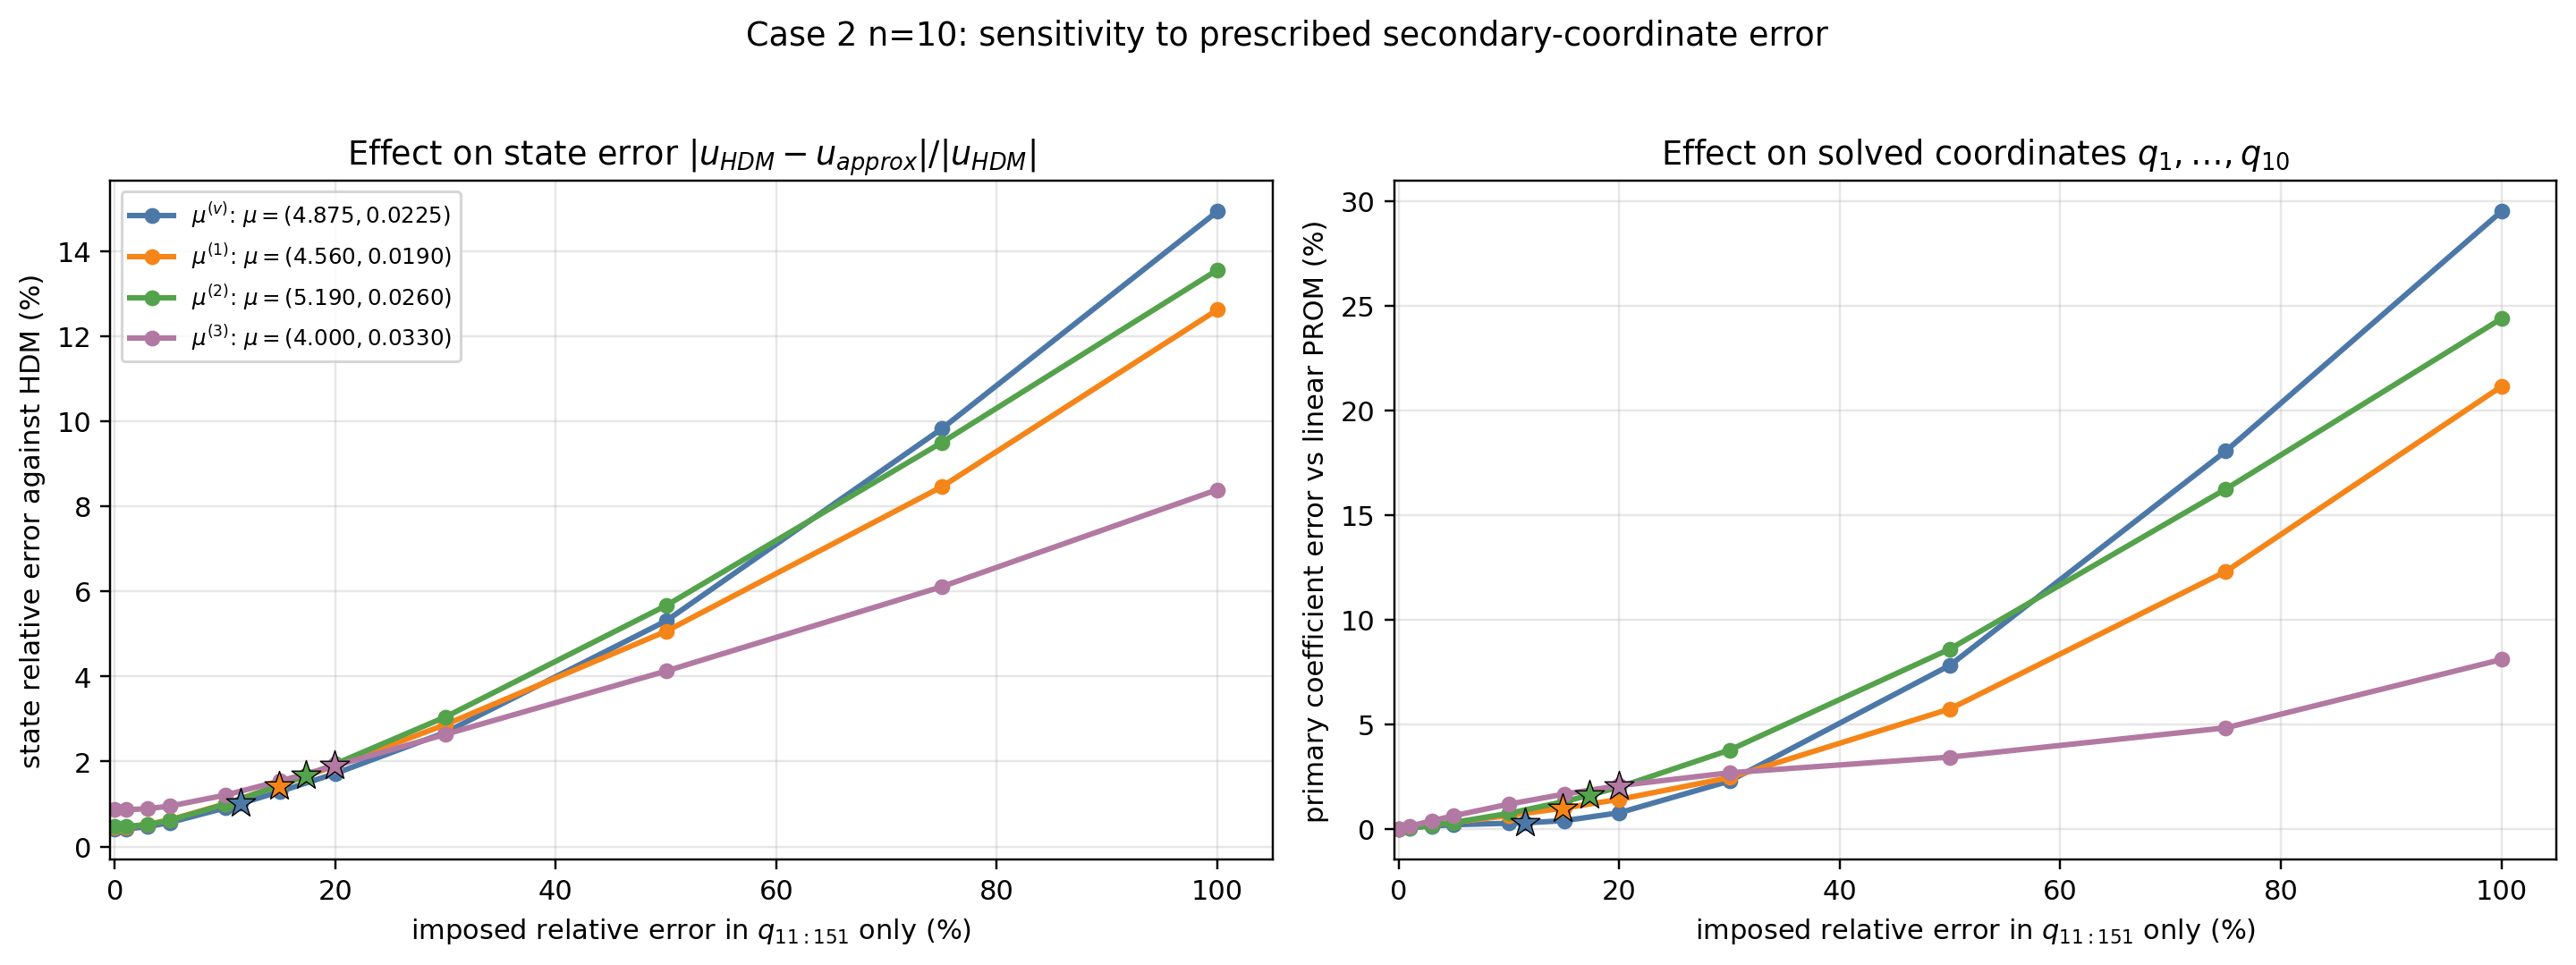
\includegraphics[width=0.98\textwidth]{figures/case2_secondary_sensitivity_state_and_primary_error.png}
\caption{Effect of the prescribed error in $q_{11},\ldots,q_{151}$ on the state error and on the recovered primary coefficients for Case~2 with $n=10$.  The horizontal axis is a secondary-block error only, not the global ANN validation error.  At zero perturbation, Case~2 uses the exact linear-PROM secondary coordinates; therefore it should recover the linear PROM lower-bound behavior up to nonlinear-solver tolerance.}
\end{figure}

\section*{Reading of the diagnostic}
The $n$-sweep tests whether solving more PROM coordinates compensates for the
master-ANN coefficient error.  The perturbation test checks the same question
more directly for fixed $n=10$: if the prescribed secondary coefficients are
made exact, the recovered primary coordinates stay close to the linear PROM
trajectory; as the secondary-coordinate perturbation grows, both the state
error and the primary-coordinate error increase.

\end{document}
